\documentclass{article}

\usepackage[utf8]{inputenc}
\usepackage{fixltx2e}
\usepackage{graphicx} 
\usepackage[a4paper, total={6in, 8in}]{geometry}
\usepackage{enumitem}
\usepackage{float}
\usepackage{subcaption}

\author{Marc Juvillà Garcia}
\title{\vspace{-2cm}Homework 1. Machine Learning (MIIS)}

\begin{document}
\maketitle

\begin{enumerate}[label=(\alph*)]
\item Generate a dataset of size 20. Plot the examples \{(x\textsubscript{n} , y\textsubscript{n})\} as well as the target function \textit{f} on a plane.
\begin{figure}[!ht]
\centering
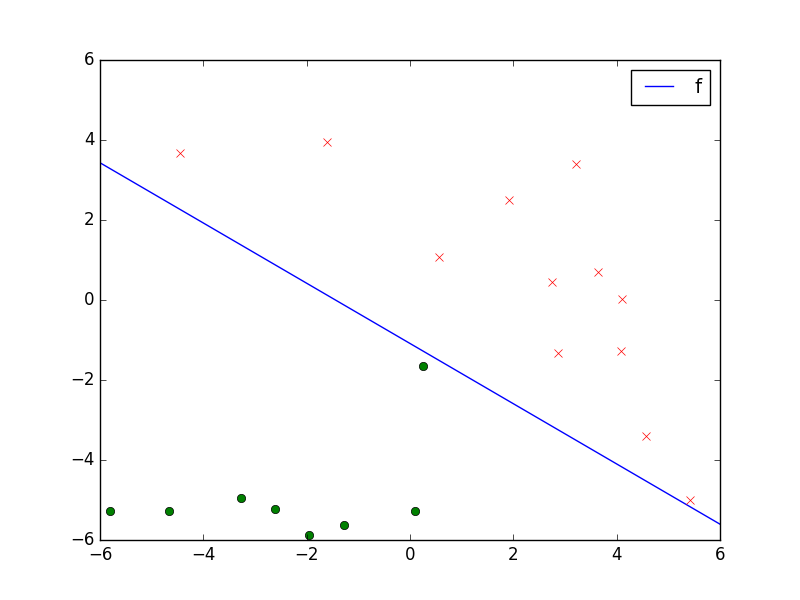
\includegraphics[scale=0.4]{images/1.png}
\caption{Dataset with 20 points with random \textit{f}.}
\end{figure}

\item Run the perceptron algorithm on the dataset. Report the number of updates that the algorithm takes before converging. Plot the examples \{(x\textsubscript{n} , y\textsubscript{n})\}, the target function \textit{f}, and the final hypothesis \textit{g} in the same figure.

\begin{figure}[H]
    \centering
    \begin{subfigure}[t]{0.5\textwidth}
        \centering
		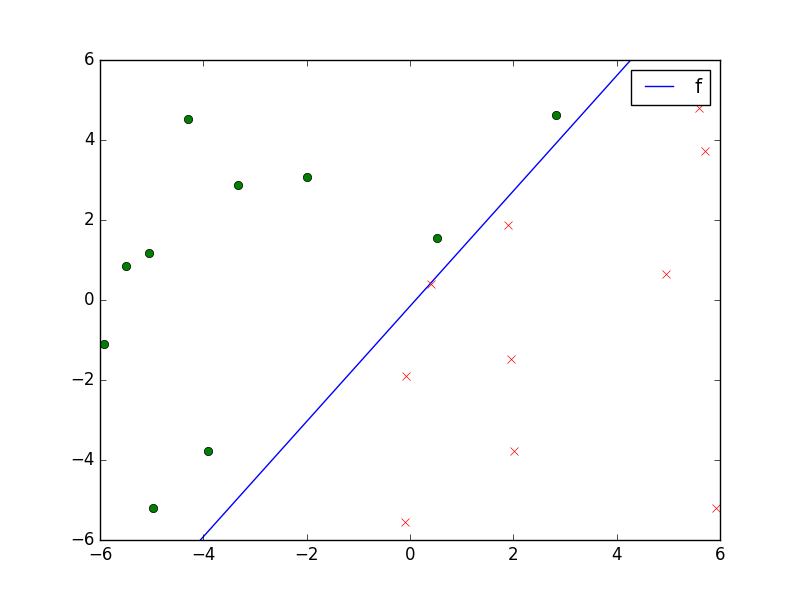
\includegraphics[scale=0.35]{images/2_a.png} 
    \end{subfigure}%
    ~ 
    \begin{subfigure}[t]{0.5\textwidth}
        \centering
		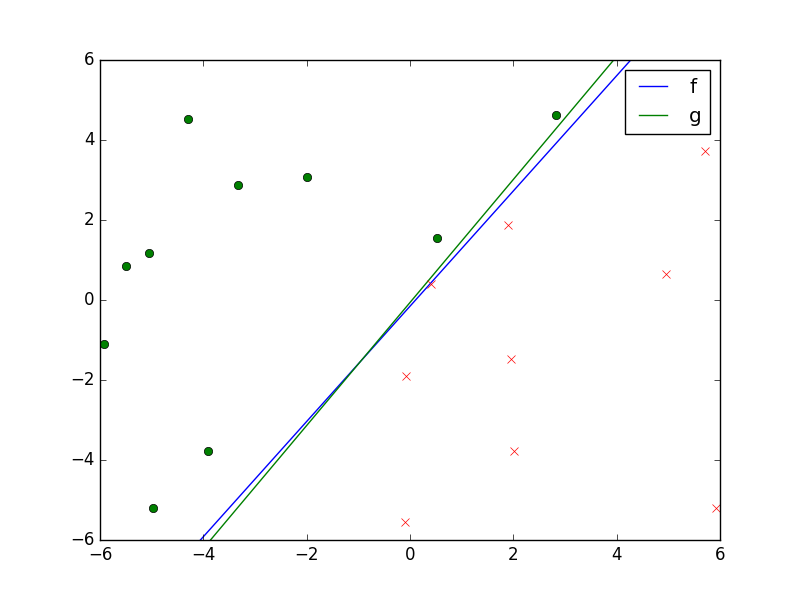
\includegraphics[scale=0.35]{images/2_b.png} 
    \end{subfigure}
    \caption{Dataset with 20 points with computed \textit{g}.}
\end{figure}

For the model shown in Figure 2, it took 12 updates of the model (that is, correcting 12 mistakes) and 0.292 ms before converging. 

\item Repeat everything in b) with another randomly generated dataset of size 20, and compare the result to b).

\begin{figure}[H]
    \centering
    \begin{subfigure}[t]{0.5\textwidth}
        \centering
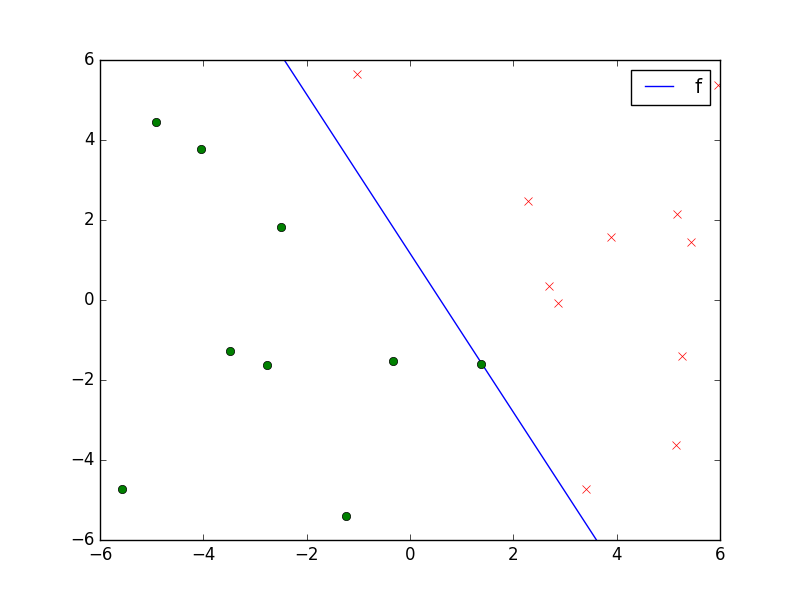
\includegraphics[scale=0.35]{images/3_a.png} 
    \end{subfigure}%
    ~ 
    \begin{subfigure}[t]{0.5\textwidth}
        \centering
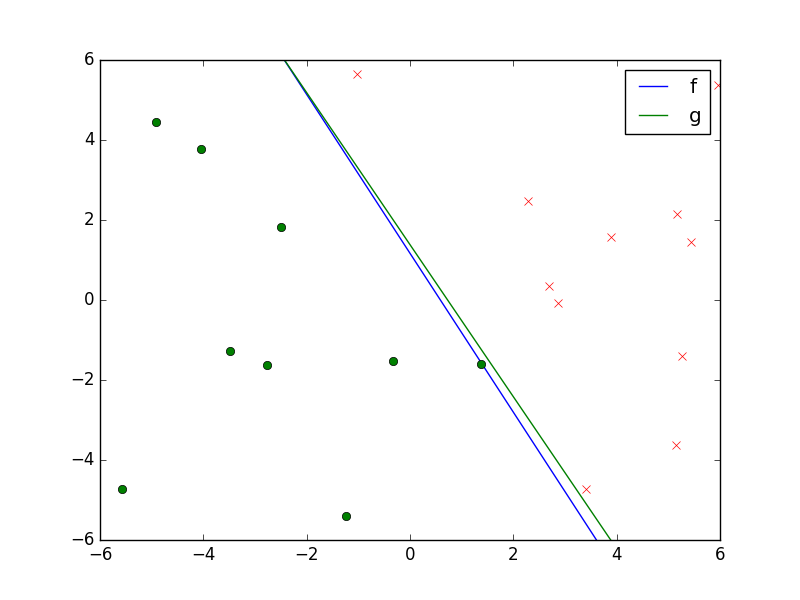
\includegraphics[scale=0.35]{images/3_b.png} 
    \end{subfigure}
    \caption{Another instance of the model of the previous question.}
\end{figure}

It took 16 updates of the model and 0.414 ms before converging, for the shown instance. \\
However, I noticed that these numbers can vary a lot so I computed the average time and update steps for 50 instances of the problem (different dataset and different \textit{f}, but same number of data points and dimension of the space), which resulted in an average of 12.2 updates and 0.218 ms.

\item Repeat everything in b) with another randomly generated dataset of size 100, and compare the result to b).

\begin{figure}[H]
    \centering
    \begin{subfigure}[t]{0.5\textwidth}
        \centering
		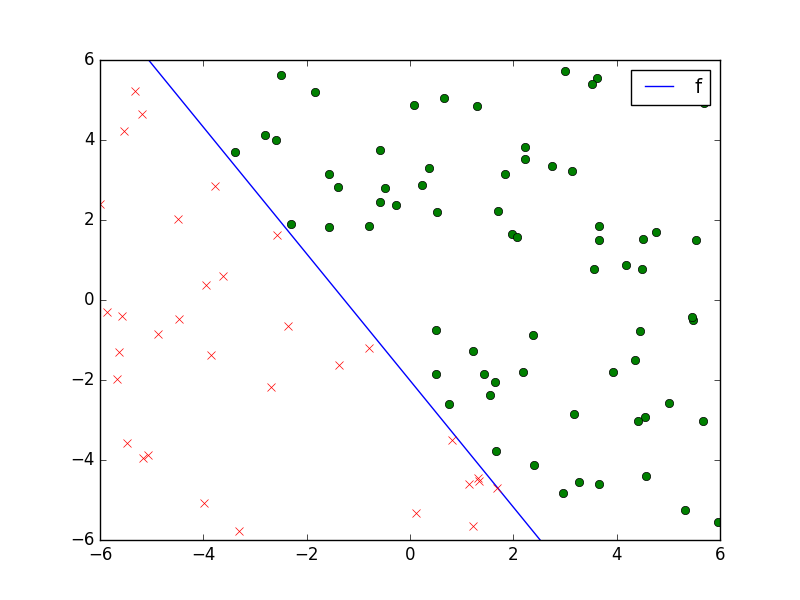
\includegraphics[scale=0.35]{images/4_a.png} 
    \end{subfigure}%
    ~ 
    \begin{subfigure}[t]{0.5\textwidth}
        \centering
		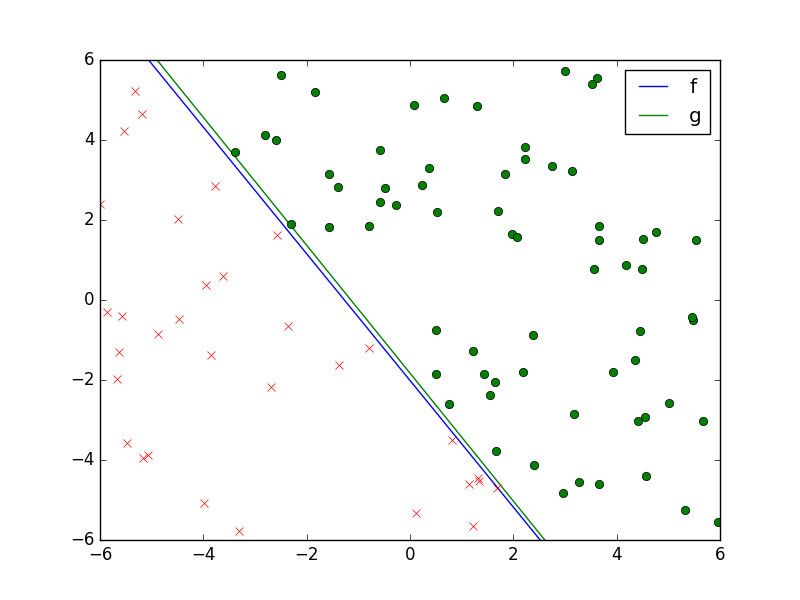
\includegraphics[scale=0.35]{images/4_b.png} 
    \end{subfigure}
    \caption{Dataset with 100 random points.}
\end{figure}

It took 78 updates of the model and 4.221 ms before converging.\\
Averaging for 50 instances of the problem, it resulted on 87.48 update steps and 2.841 ms of training time.\\
Comparing these results to the ones in section b, we see that the update steps have increased by a factor of $\sim$7, and the training time by $\sim$13.

\item Repeat everything in b) with another randomly generated dataset of size 1000, and compare the result to b).

\begin{figure}[H]
    \centering
    \begin{subfigure}[t]{0.5\textwidth}
        \centering
		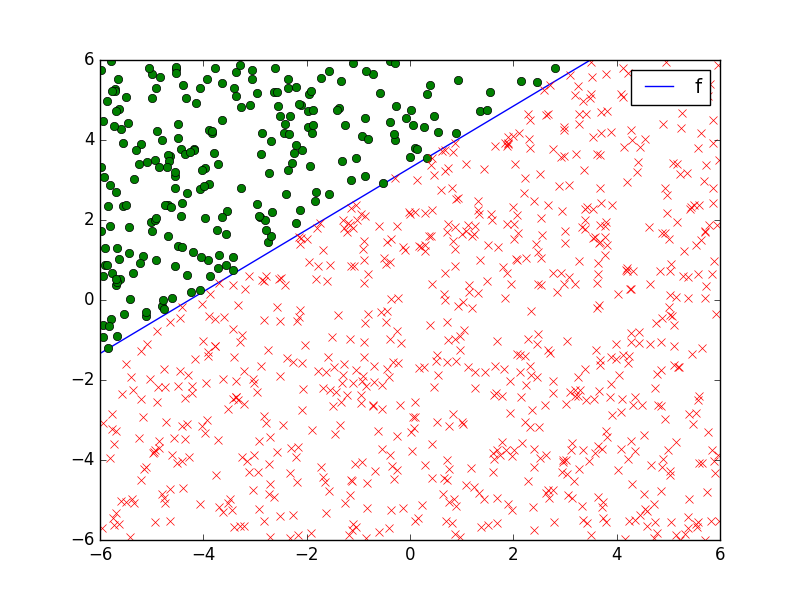
\includegraphics[scale=0.35]{images/5_a.png} 
    \end{subfigure}%
    ~ 
    \begin{subfigure}[t]{0.5\textwidth}
        \centering
		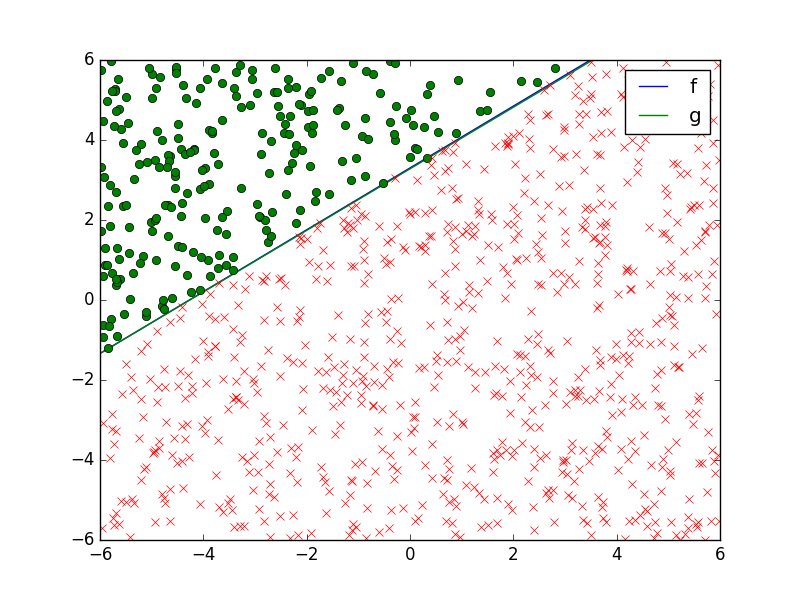
\includegraphics[scale=0.35]{images/5_b.png} 
    \end{subfigure}
    \caption{Dataset with 1000 random points.}
\end{figure}

It took 2176 updates of the model and 195.669 ms before converging.\\
Averaging for 50 instances of the problem, it resulted on 452.7 update steps and 50.815 ms of training time.
Comparing these results to the ones in section b, we see that the update steps have increased by a factor of $\sim$37, and the training time by $\sim$233.\\
Compared to the results of section d, multiplying by 10 the number of samples results in an increase by $\sim$5 of the number of update steps and by $\sim$18 of the processing time.

\item Modify the experiment such that x\textsubscript{n}$\in$R\textsuperscript{10} instead of R\textsuperscript{2} . Run the algorithm on a randomly generated dataset of size 1000. How many updates does the algorithm take to converge?

It took 6529 updates of the model and 979.125 ms before converging.\\
Averaging for 50 instances of the problem, it resulted on 5908.7 update steps and 737.511 ms of training time.

\item Summarize your conclusions regarding the accuracy and running time of the algorithm as a function of N (the number of data points) and d (the number of dimensions).\\\\
The following table summarizes the results of the previous sections.

\begin{table}[H]
{\centering
\resizebox{\textwidth}{!}{%
\begin{tabular}{lcccc}
\hline
\multicolumn{1}{c}{} & \multicolumn{1}{l}{N = 20; d = 2} & \multicolumn{1}{l}{N = 100; d = 2} & \multicolumn{1}{l}{N = 1000; d = 2} & \multicolumn{1}{l}{N = 1000; d = 10} \\ \hline
Steps                & 12.2                              & 87.48                              & 452.7                               & 5908.7                               \\ \hline
Time (ms)            & 0.218                             & 2.841                              & 50.815                              & 737.511                              \\ \hline

\end{tabular}%
}}
\caption{Summarized results.}
\end{table}


In terms of accuracy, given that the two classes are linearly separable (we made it that way when generating the datasets), the perceptron training algorithm always finds the perfect boundary, so the accuracy is 1.\\
In terms of speed, we can see an increase of time steps when the number of samples is increased, and a stronger increase when we increment the dimension of the space. The following figures try to illustrate this effect.

\begin{figure}[H]
    \centering
    \begin{subfigure}[t]{0.5\textwidth}
        \centering
		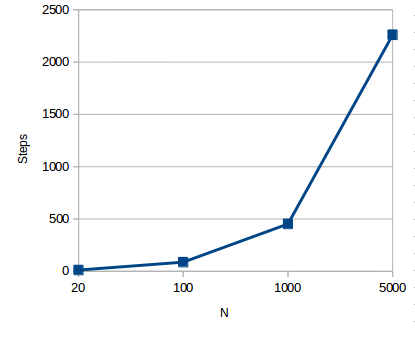
\includegraphics[scale=0.5]{images/6_a.png} 
    \end{subfigure}%
    ~ 
    \begin{subfigure}[t]{0.5\textwidth}
        \centering
		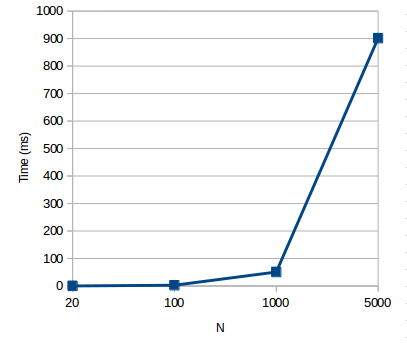
\includegraphics[scale=0.5]{images/6_b.png} 
    \end{subfigure}
    \caption{Exponential increase of number of steps and processing time (d=2)}
\end{figure}

\begin{figure}[H]
    \centering
    \begin{subfigure}[t]{0.5\textwidth}
        \centering
		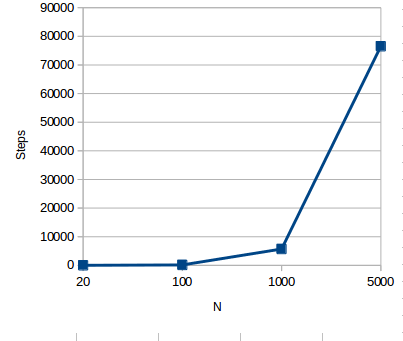
\includegraphics[scale=0.5]{images/6_c.png} 
    \end{subfigure}%
    ~ 
    \begin{subfigure}[t]{0.5\textwidth}
        \centering
		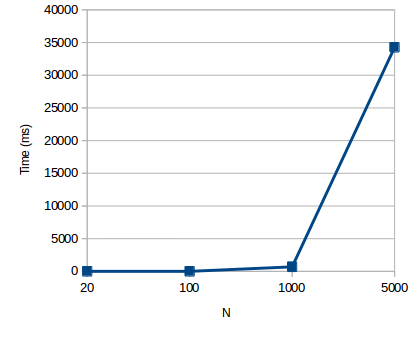
\includegraphics[scale=0.5]{images/6_d.png} 
    \end{subfigure}
    \caption{Exponential increase of number of steps and processing time (d=10)}
\end{figure}

As can be seen in the attached figures, both models present an exponential increase in its number of steps amb processing time when incrementing the data points, but this effect is stronger with more dimensions.\\

In summary, it was foreseeable that the processing time was going to increment when adding data points to the dataset or adding dimensions to the space - the more data points, the more (statistically) errors to correct; the more dimensions, the more processing time when computing the perceptron parameters. \\

Speaking about accuracy, in general terms adding training samples to the dataset helps the training algorithm to generalize better and by extension to avoid overfitting, while adding dimensions to the training samples tends to make the dataset more sparse and so easier to separate in classes. For this reason, we need to find a trade-off between the accuracy and the processing time, adjusting the parameters of the model.

\end{enumerate}


\end{document}
